\documentclass{article}
\usepackage[english]{babel}
\usepackage[usenames,dvipsnames]{color}
\usepackage{amssymb}
\usepackage{amsmath}
\usepackage{cases}
\usepackage{url}
\usepackage{mathrsfs}
\usepackage{multirow}
\usepackage{booktabs}
\usepackage{rotating}
\usepackage{graphicx}
\usepackage[maxnames=5, sorting=none, defernumbers=true]{biblatex}
\usepackage{csquotes}
\usepackage{flushend}

\makeatletter
\let\l@ENGLISH\l@english
\makeatother

%
% Submission and revision
%
\usepackage{pdfpages}

\definecolor{updated}{rgb}{1,0,0}
\definecolor{updatedBackground}{rgb}{1,0.95,0.95}

\usepackage[normalem]{ulem}
\newcommand{\updated}[1]{{\color{updated}\uline{#1}}}

\newcommand{\updatedFigure}[1]{%
  \setlength{\fboxsep}{0pt}%
  \setlength{\fboxrule}{1pt}%
  \vspace*{-2pt}%
  \hspace*{-5pt}%
  \fcolorbox{updated}{updatedBackground}{#1}%
}

\AtEveryBibitem{%
  \iffieldequalstr{note}{updated}
  {%
    \clearfield{note}%
    \color{red}%
  }%
  {%
  }%
}

%
% Fonts
%
\newcommand*{\TitleFont}{%
  \fontsize{22}{26}%
  \selectfont%
}

\renewcommand*{\bibfont}{\small}

%
% References
%
\newcommand{\eref}[1]{Eq.~(\ref{equ:#1})}
\newcommand{\sref}[1]{Sec.~\ref{sec:#1}}
\newcommand{\aref}[1]{App.~\ref{app:#1}}
\newcommand{\tref}[1]{Tab.~\ref{tab:#1}}
\newcommand{\fref}[1]{Fig.~\ref{fig:#1}}

\newcommand{\elabel}[1]{\label{equ:#1}}
\newcommand{\slabel}[1]{\label{sec:#1}}
\newcommand{\alabel}[1]{\label{app:#1}}
\newcommand{\tlabel}[1]{\label{tab:#1}}
\newcommand{\flabel}[1]{\label{fig:#1}}

%
% Text shortcuts
%
\newcommand{\cdf}{CDF}
\newcommand{\cdfs}{CDFs}
\newcommand{\pdf}{PDF}
\newcommand{\pdfs}{PDFs}
\newcommand{\nrmse}{NRMSE}
\newcommand{\nrmses}{NRMSEs}

\newcommand{\ie}{\emph{i.e.}}
\newcommand{\eg}{\emph{e.g.}}
\newcommand{\etc}{\emph{etc.}}
\newcommand{\apriori}{\emph{a priori}}
\newcommand{\versus}{vs.}
\newcommand{\via}{via}
\newcommand{\etal}{\emph{et al.}}

\makeatletter
\def\stage#1{\@ifnextchar\bgroup{\stageDouble{#1}}{\stageSingle{#1}}}
\def\stageSingle#1{\textbf{Stage~#1}}
\def\stageDouble#1#2{\textbf{Stage~#1.}\hspace{0.5em}\emph{#2}}
\makeatother

%
% Tables
%
\usepackage{array}
\newcolumntype{L}[1]{>{\raggedright\let\newline\\\arraybackslash\hspace{0pt}}m{#1}}
\newcolumntype{C}[1]{>{\centering\let\newline\\\arraybackslash\hspace{0pt}}m{#1}}
\newcolumntype{R}[1]{>{\raggedleft\let\newline\\\arraybackslash\hspace{0pt}}m{#1}}

\newcolumntype{=}{>{\global\let\currentrowstyle\relax}}
\newcolumntype{-}{>{\currentrowstyle}}
\newcommand{\rowstyle}[1]{\gdef\currentrowstyle{#1}%
  #1\ignorespaces
}

\newcommand{\eExp}{\epsilon_\mathbb{E}}
\newcommand{\eVar}{\epsilon_{\mathbb{V}\text{ar}}}
\newcommand{\ePDF}{\epsilon_\fPDF}

\newcommand{\colExp}{$\eExp, \%$}
\newcommand{\colVar}{$\eVar, \%$}
\newcommand{\colPDF}{$\ePDF, \%$}
\newcommand{\colMC}[1]{$\scriptstyle \nsamples = 10^#1$}

%
% Spaces
%
\renewcommand{\L}[1]{\mathcal{L}_{#1}}
\newcommand{\real}{\mathbb{R}}

%
% Linear algebra
%
\newcommand{\m}[1]{\mathbf{\MakeUppercase{#1}}}

\newcommand{\mI}{\m{I}}
\newcommand{\mZero}{\m{0}}

\renewcommand{\vec}[1]{\left(#1\right)^T}
\renewcommand{\v}[1]{\mathbf{#1}}

\newcommand{\vZero}{\v{0}}

\newcommand{\abs}[1]{| #1 |}
\newcommand{\norm}[1]{\| #1 \|}

%
% Probability theory
%
\newcommand{\outcomes}{\Omega}
\renewcommand{\o}{\omega}
\newcommand{\sAlgebra}{\mathcal{F}}
\newcommand{\pMeasure}{\mathbb{P}}

\newcommand{\dBeta}{\text{Beta}}

\newcommand{\vExp}{{\boldsymbol\mu}}
\newcommand{\mCov}{\m{\Sigma}}

\newcommand{\oExp}[1]{\mathbb{E}\left(#1\right)}
\newcommand{\oVar}[1]{\mathbb{V}\text{ar}\left(#1\right)}
\newcommand{\oCov}[1]{\mathbb{C}\text{ov}\left(#1\right)}
\newcommand{\oCorr}[1]{\mathbb{C}\text{orr}\left(#1\right)}

\newcommand{\SE}{\text{SE}}
\newcommand{\OU}{\text{OU}}

\newcommand{\fPDF}{f}
\newcommand{\fCDF}{F}

\newcommand{\oNataf}[1]{\mathcal{N}\left[#1\right]}
\newcommand{\oInvNataf}[1]{\mathcal{N}^{-1}\left[#1\right]}

\makeatletter
\def\fMean{\@ifnextchar\bgroup{\fMeanOne}{\fMeanZero}}
\def\fMeanOne#1{\mu(#1)}
\def\fMeanZero{\mu}

\def\fCov{\@ifnextchar\bgroup{\fCovOne}{\fCovZero}}
\def\fCovOne#1{k(#1)}
\def\fCovZero{k}

\def\fCorr{\@ifnextchar\bgroup{\fCorrOne}{\fCorrZero}}
\def\fCorrOne#1{k(#1)}
\def\fCorrZero{k}
\makeatother

%
% Polynomial chaos expansion
%
\newcommand{\pcb}{\Phi}
\newcommand{\pcn}{\eta}
\newcommand{\pcc}[1]{\hat{#1}}
\newcommand{\oPC}[3]{\mathcal{C}_{#1}^{#2}\left[#3\right]}

\makeatletter
\def\oInner#1{\@ifnextchar\bgroup{\oInnerDouble{#1}}{\oInnerSingle{#1}}}
\def\oInnerSingle#1{\left\langle #1 \right\rangle}
\def\oInnerDouble#1#2{\oInnerSingle{#1, #2}}
\makeatother

%
% Karhunen-Loeve expansion
%
\newcommand{\domain}{\mathcal{D}}
\newcommand{\klv}{\lambda}
\newcommand{\klf}[1]{\hat{#1}}
\newcommand{\mKL}{\m{K}}

%
% Integration with quadratures
%
\newcommand{\qdn}[1]{\hat{#1}}
\newcommand{\qdw}{w}
\newcommand{\oQuad}[3]{\mathcal{Q}_{#1}^{#2}\left[#3\right]}

%
% Thermal model:
%
%      dT
%  C * -- + (G - G_amb) * T = P
%      dt
%

% Specification
\newcommand{\system}{\mathcal{S}}

% Capacitance and conductance
\newcommand{\mC}{\m{C}}
\newcommand{\mG}{\m{G}}

%
% Transformed thermal model:
%
%  dX
%  -- = A * X + B * P
%  dt
%
%  Y = B^T * X
%
\newcommand{\vX}{\v{X}}
\newcommand{\mA}{\m{A}}
\newcommand{\mB}{\m{B}}

% Processor elements/thermal nodes mapping
\newcommand{\mM}{\m{\tilde{B}}}

% Recurrence coefficients
\newcommand{\mCF}{\m{D}}
\newcommand{\mCS}{\m{E}}

%
% Time
%
\renewcommand{\t}{t}
\newcommand{\dt}{\Delta \t}
\newcommand{\period}{T}
\newcommand{\sTime}{T}

%
% Temperature
%
\newcommand{\T}{Q}
\newcommand{\vTI}{\v{\tilde{Q}}}
\newcommand{\vTO}{\v{\T}}
\newcommand{\mTO}{\m{\T}}

\newcommand{\amb}{\text{amb}}

%
% Power
%
\renewcommand{\P}{P}
\newcommand{\vP}{\v{P}}
\newcommand{\mP}{\m{P}}

\newcommand{\dyn}{\text{dyn}}
\newcommand{\leak}{\text{leak}}
\newcommand{\stat}{\text{stat}}

\newcommand{\f}{f}

\makeatletter
\def\oPower{\@ifnextchar\bgroup{\oPowerPlus}{\oPowerZero}}
\def\oPowerPlus#1{\@ifnextchar\bgroup{\oPowerTwo{#1}}{\oPowerOne{#1}}}
\def\oPowerTwo#1#2{\Pi_{#1}\left(#2\right)}
\def\oPowerOne#1{\Pi\left(#1\right)}
\def\oPowerZero{\Pi}
\makeatother

%
% System profiles
%
\newcommand{\profile}[1]{( #1, \partition{#1} )}
\newcommand{\partition}[1]{\tau[#1]}

\makeatletter
\def\profileP{\@ifnextchar\bgroup{\profilePWithArgument}{\profilePWithoutArgument}}
\def\profilePWithArgument#1{\profile{\mP(#1)}}
\def\profilePWithoutArgument{\profile{\mP}}

\newcommand{\profilePdyn}{(\mP_\dyn, \partition{\mP_\dyn})}

\def\profileT{\@ifnextchar\bgroup{\profileTWithArgument}{\profileTWithoutArgument}}
\def\profileTWithArgument#1{\profile{\mTO(#1)}}
\def\profileTWithoutArgument{\profile{\mTO}}
\makeatother

%
% Uncertain parameters
%
\newcommand{\U}{U}
\newcommand{\vU}{\v{U}}

%
% Independent random variables
%
\newcommand{\z}{\zeta}
\newcommand{\Z}{Z}
\newcommand{\vZ}{\v{Z}}
\newcommand{\vz}{\boldsymbol{\zeta}}

\makeatletter
\def\oTransform{\@ifnextchar\bgroup{\oTransformWithArgument}{\oTransformWithoutArgument}}
\def\oTransformWithArgument#1{\mathcal{T}\left[#1\right]}
\def\oTransformWithoutArgument{\mathcal{T}}
\makeatother

%
% Process variation
%
\newcommand{\Leff}{L}
\newcommand{\vLeff}{\v{L}}
\newcommand{\nLeff}{L}
\newcommand{\gLeff}{{\delta L^{(g)}}}
\newcommand{\lLeff}{\delta L^{(l)}}
\newcommand{\vlLeff}{\delta \v{L}^{(l)}}

\renewcommand{\r}{r}
\newcommand{\vr}{\v{r}}

%
% Numbers
%
\newcommand{\nnodes}{{n_\text{n}}}
\newcommand{\nprocs}{{n_\text{p}}}
\newcommand{\nsteps}{{n_\text{t}}}

\newcommand{\nvars}{{n_\text{v}}}

\newcommand{\pcorder}{{n_\text{po}}}
\newcommand{\pcterms}{{n_\text{pt}}}

\newcommand{\qdlevel}{{n_\text{ql}}}
\newcommand{\qdorder}{{n_\text{qo}}}
\newcommand{\qdorderone}{{\tilde{n}_\text{qo}}}
\newcommand{\qdprecision}{{n_\text{qp}}}

\newcommand{\nsamples}{{n_\text{mc}}}


\usepackage{anysize}
\usepackage[a4paper,top=29mm,bottom=30mm,left=30mm,right=30mm]{geometry}

\usepackage{mdframed,color}

\definecolor{done}{rgb}{0,0,1}
\definecolor{reviewerLine}{rgb}{0.1,0.1,0.1}
\definecolor{reviewerBackground}{rgb}{0.95,0.95,1}

\mdfdefinestyle{reviewer}{%
  leftmargin=0cm,%
  rightmargin=0cm,%
  innerleftmargin=1em,%
  innerrightmargin=1em,%
  linecolor=reviewerLine,%
  backgroundcolor=reviewerBackground%
}

\newenvironment{reviewer}{%
  \begin{mdframed}[style=reviewer]%
}{%
  \end{mdframed}%
  \vspace{1.0em}%
}
\newenvironment{authors}{%
}{%
  \vspace{1.0em}%
}

\newcommand{\perse}{\emph{per se}}

\newcommand{\done}[1]{%
  {\color{done}$\checkmark$~\uline{#1}}%
}

\newcommand{\figureBox}[1]{%
  \fcolorbox{updated}{updatedBackground}{#1}%
}

\newcommand{\reviewerBox}[1]{%
  \fcolorbox{reviewerLine}{reviewerBackground}{#1}%
}

\begin{document}
  \pagenumbering{gobble}

  \begin{titlepage}
    \section*{\hspace{6em}{\Huge Submission Notes}}
    \vspace{1em}
    \linespread{1.1}
    \Large
    No part of this work, titled ``Probabilistic Analysis of Power and Temperature Under Process Variation for Electronic System Design'' by I. Ukhov \etal, has been published before as part of any conference or journal paper.
  \end{titlepage}

  \section*{\hspace{3em}{\Huge Response to the Reviewers}}

  \section*{General Notes}
  Dear Reviewers,
  \\
  \\
  \\
  \noindent Thank you for your time and valuable feedback.
  Please find below our response to your comments.
  The text of the comments is placed in \reviewerBox{boxes} with dark gray borders and pale blue backgrounds.
  Each such box is followed by our reply and a short summary of the taken actions given as a \done{checklist} highlighted with blue color and underlined.
  In the manuscript, the new and updated parts are \updated{marked} with red color and underlined.
  The changed figures are placed in \figureBox{boxes} with red borders and pale red backgrounds.
  Due to the limitation of space, three figures have been removed from the paper, namely, Fig.~4, depicting the first six polynomials of the Hermite basis, Fig.~5, illustrating a beta fit to the standard Gaussian distribution, and Fig.~10, comparing full-tensor product and sparse integration grids.
  \\
  \\
  \\
  \noindent Sincerely yours,\\
  Ivan Ukhov, Petru Eles, and Zebo Peng

  \section*{Reviewer 1}
  \begin{reviewer}
This paper proposed a novel approach to model transient power-temperature behavior considering process variation. This is a missing piece in statistical power/temperature analysis due to many reasons and technical difficulties. I think the proposed solution may still have some limitations and assumptions, but it has big contribution to the area, and one step closer to practical usage. Experiments are sufficient to validate the proposed framework. The paper is well written and organized as well.
\end{reviewer}
\begin{authors}
Thank you for the kind words.
\end{authors}

\begin{reviewer}
This is an interesting topic, so some of my comments are more like discussions:

1) Power consumption has two components: dynamic power and leakage power. Process variation mainly affects leakage power. I think that’s why the authors focus on the model for statistical leakage power. However, temperature and total power (dynamic and leakage) are highly correlated. Since this paper is focus on modeling transient power-temperature behavior, the accuracy of total power model is important. Dynamic power is related to the run-time operations. In Sec. VII, the dynamic power profiles are obtained by simulations of randomly generated via TGFF, applications defined by DAGs of tasks. Usually the simulation has a size limit, it will be nice to provide some details about how large scale of the chip can be.
\end{reviewer}
\begin{authors}
The workload to be analyzed is an input to our framework without any further restrictions: it is arbitrary and can come from an arbitrary source.
Therefore, it would not make much contribution to the paper if we performed, for example, cycle-accurate simulations of some real-life applications and used the output of these simulation as an input to our analysis.
Instead, our applications are generated randomly via TGFF.
Apart from a DAG, TGFF generates a set of tables that specify the execution time and dynamic power of each task for each processing element individually.
Then the simulation that we perform consists of a scheduling procedure of the DAG, which determines when and where each task should be executed (we employ a list scheduler for this purpose).
Once this has been decided, the corresponding dynamic power profile is constructed based on the tables provided by TGFF.
The output files of TGFF used in our experiments are available online.

In practice, of course, dynamic power profiles should be properly captured using adequate simulators capable of modeling the power dissipation.
In particular, the following interrelated tools are very frequently used for this purpose: SimpleScalar, PTscalar, gem5, McPAT, and Wattch.
As Reviewer~2 pointed out in the second comment, contemporary software packages can address ``[\ldots] fairly big size examples and circuits.''

\done{The input workload has been detailed further, Sec.~IV.}

\done{Practical aspects of the input workload have been outlined in Sec.~VII.}
\end{authors}

\begin{reviewer}
2) Question about the thermal model: The authors mentioned the following in Sec. IV-C: ``Given the thermal specification S of the system at hand (see Sec. IV), \ldots'' I’m interested in the modeling of thermal specification as well. But it seems that the authors are referring to the wrong Section (or should provide more details about sub-session?).
\end{reviewer}
\begin{authors}
The specification $\system$ is a shortcut for us to refer to all the information needed for the construction of an equivalent thermal RC circuit of the system.
The content of $\system$ is described in the second paragraph of Sec. IV, and it is specific to the way the RC circuit is obtained.
In our experiments, we utilize the block model of HotSpot v5.02 for this purpose.
$\system$ then reflects the configuration of HotSpot, which includes more than 60 parameters such as the chip thickness, silicon thermal conductivity, silicon specific heat, \etc\ Please refer to ``Temperature-aware Microarchitecture: Modeling and Implementation'' by K. Skadron \etal\ for further details.

\done{The reference to $\system$ from Sec.~V-C has been improved.}

\done{The content of $\system$ has been detailed further, Sec.~IV.}

\done{Two references, namely, [Kreith, 2000] ([22] in the previous version) and [HotSpot] ([31] in the previous version), have been replaced by [Skadron, 2004], mentioned above, which is more concrete and well suited for the discussions in the paper.}
\end{authors}

\begin{reviewer}
In Sec. III, the authors mentioned that this framework works for electronic systems with temperature profiles. Is that chip level? Architecture level? If it’s chip level, the cooling system is not settled yet, so it’s hard to have a final temperature profile;
\end{reviewer}
\begin{authors}
The thermal modeling considered in this paper is at the architecture/system level.
The cooling system is assumed to be settled in order to construct an adequate thermal RC circuit.
Therefore, the thermal package is included in the thermal model, as mentioned in the second paragraph of Sec.~IV.
To elaborate, the thermal package in the experimental results consists of three layers: the thermal interface material, heat spreader, and heat sink.
Unfortunately, due to the shortage of space, we no longer have an illustration of such a circuit with a thermal package in the paper.
However, we would like to give it here.
\begin{figure}[!h]
  \centering
  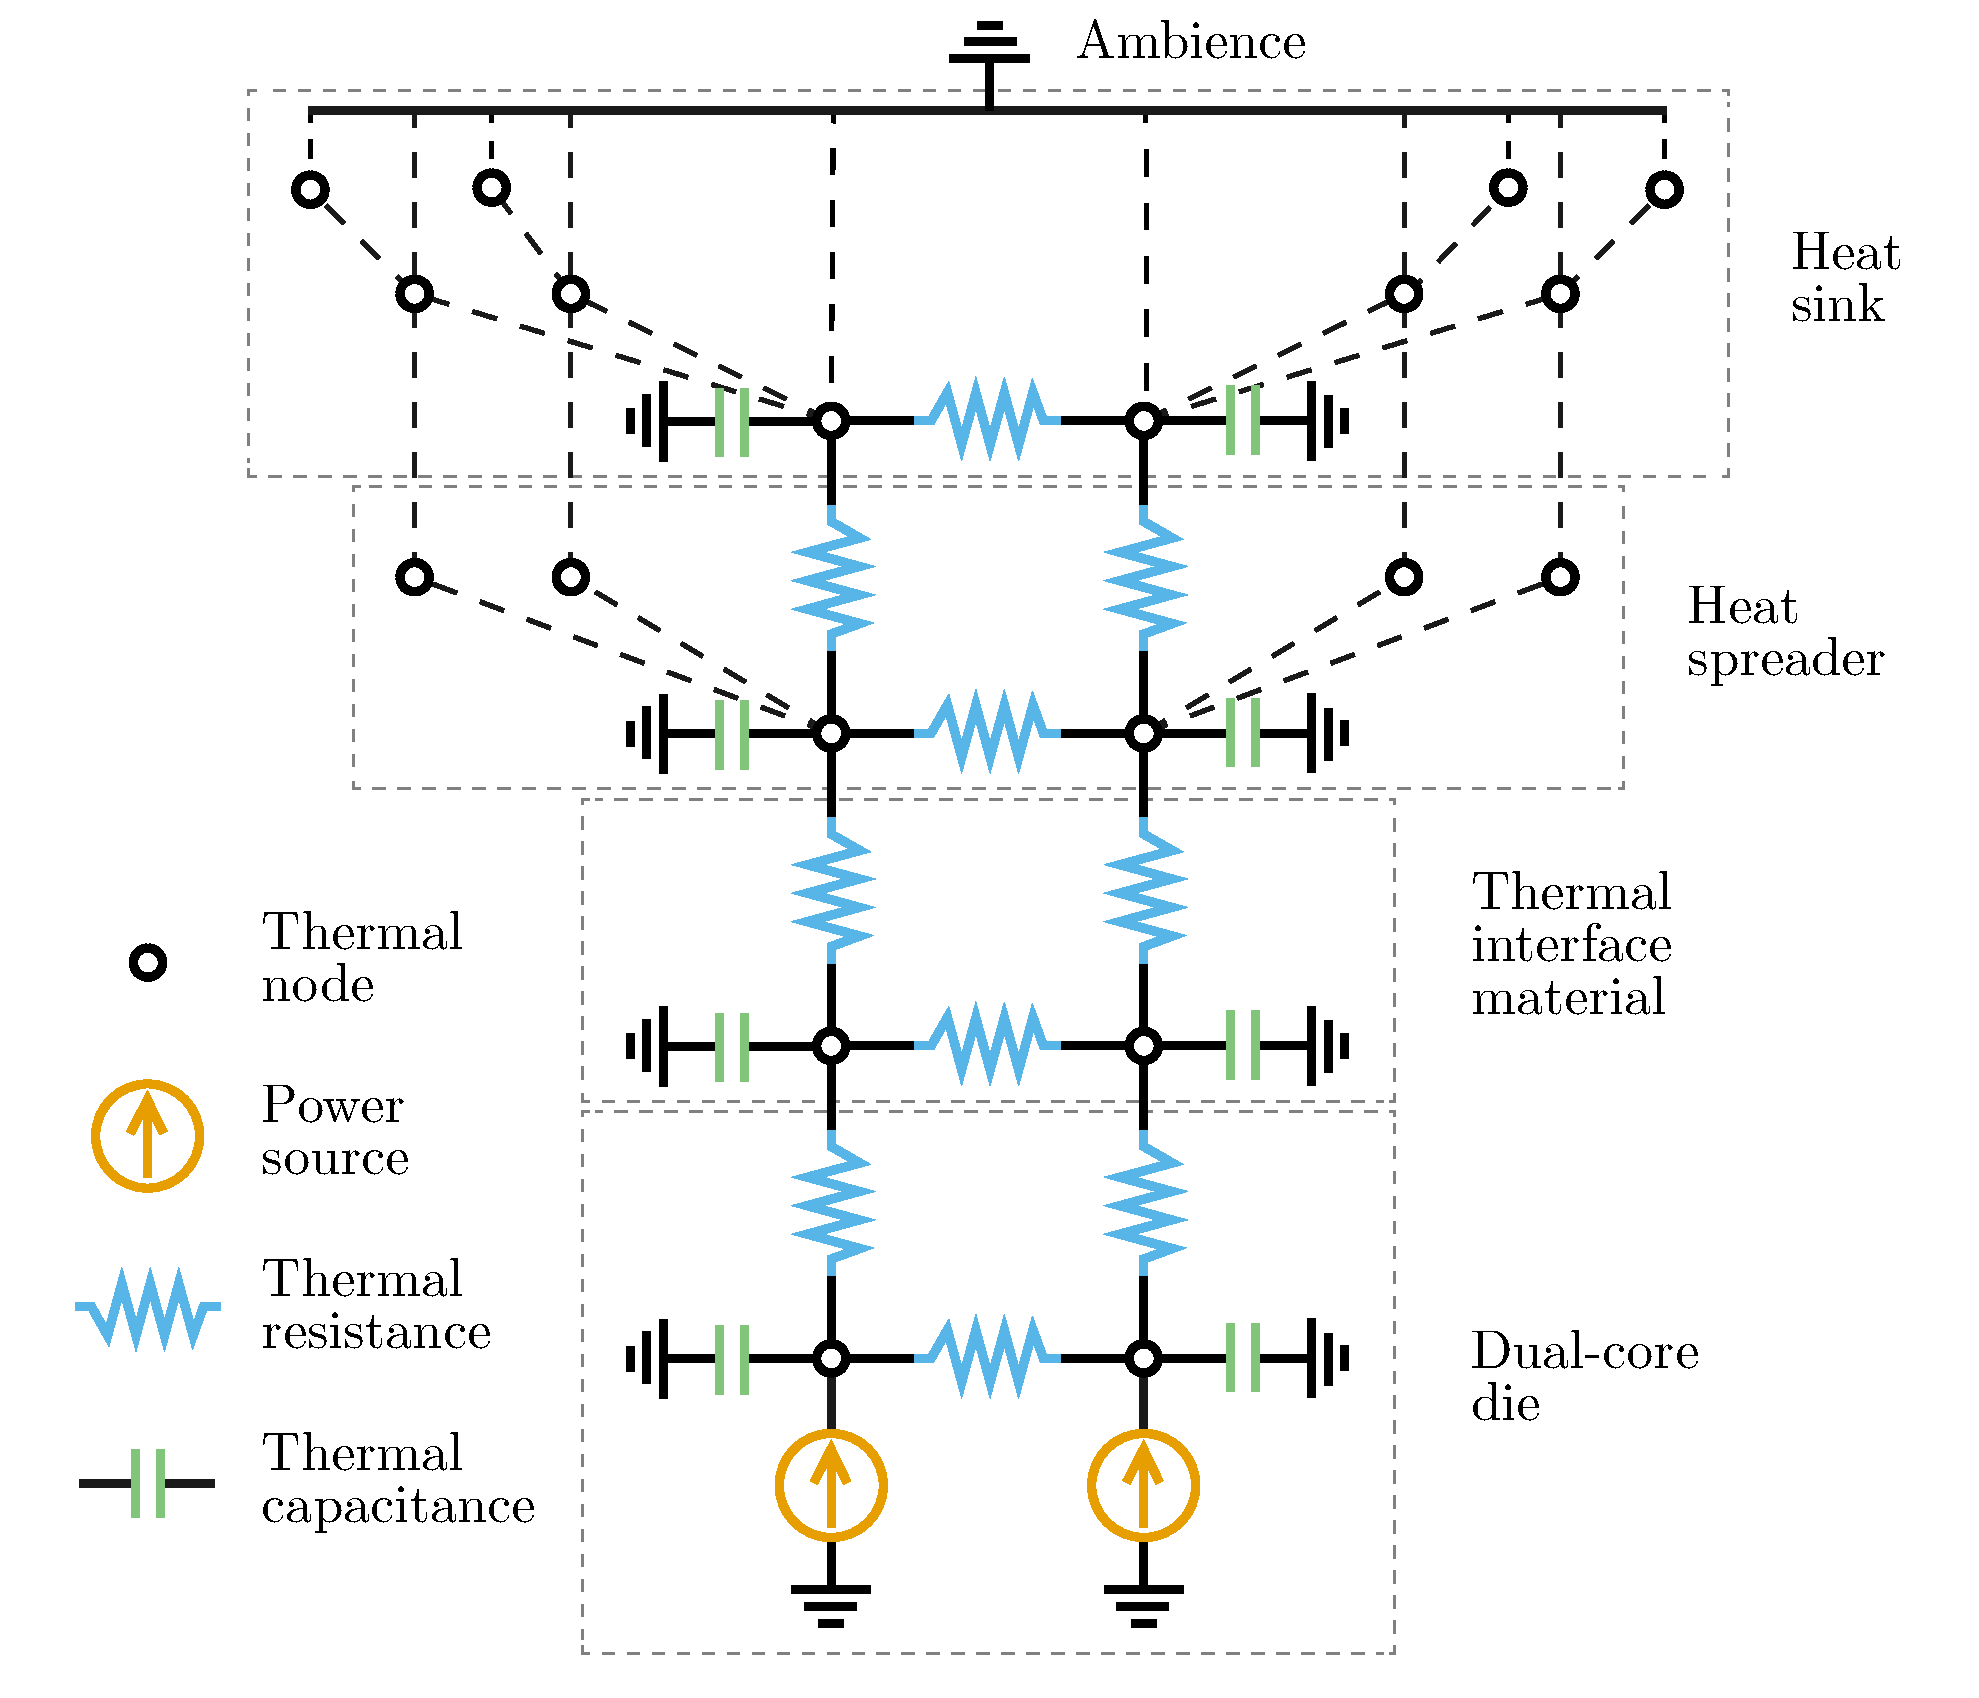
\includegraphics[width=0.5\linewidth]{include/assets/circuit.pdf}
  \vspace{-0.5em}
  \caption{A simplified thermal RC circuit for a dual-core platform.}
  \flabel{circuit}
\end{figure}

The top three dashed boxes in \fref{circuit} correspond to the aforementioned three layers.

\done{The system-level scope of the paper has been emphasized in Sec.~IV.}
\end{authors}

\begin{reviewer}
If it’s architecture level, there might be multiple chips involved with different statistical power behaviors, I’m curious about how the proposed method works in this situation.
\end{reviewer}
\begin{authors}
The source of uncertainty considered in this work is process variation.
At the design stage, the process parameters of a yet-to-be-fabricated chip are random variables.
Once the chip has been fabricated, these parameters take particular values and remain fixed hereafter, \ie, the process parameters of this particular chip become deterministic.
Thus, a \emph{fabricated} chip does \emph{not} exhibit any statistical behavior; the behavior is deterministic.
However, since this behavior is unknown at the design stage, the power/temperature profiles are stochastic for the designer, and our framework provides with the tools to characterizes all possible outcomes of these uncertain profiles.

\done{The above discussion has been included in Sec.~IV.}
\end{authors}

\begin{reviewer}
3) On Fig 1, it will be nice to use different line shapes as well. When the paper is printed black/white, it’s hard to tell the color difference.
\end{reviewer}
\begin{authors}

\done{Fig.~1 have been adapted for printing in grayscale.}

\done{The same issue has been addressed regarding Fig.~3, Fig.~4, Fig.~5, and Fig.~6.}
\end{authors}


  \section*{Reviewer 2}
  \begin{reviewer}
Using polynomial chaos (PC) approach to capture process variation caused performance issues in VLSI design was first pointed out and developed by authors from [5][17][18]. And it really works well ! Most theoretical part of this paper followed similar derivations as these previous papers. However, comparing with Monte Carlo based approaches, PC may end up doing  lengthy  coefficients solving procedure. No surprise that the authors need additional surrogate modeling and multi-processors to deal with the speedup.

This paper is well written overall.
\end{reviewer}
\begin{authors}
Thank you.
\end{authors}

\begin{reviewer}
My major concerns are in the experimental results part.

1) The authors used 45nm technology node. But the variation is only 5\%. Is this too low ? Of course variations depend on fab. Different companies may provide different number. But isnt this should be around 30\% to 50\% on average.
\end{reviewer}
\begin{authors}
We would like to begin by noting that our framework is not constrained by any particular value of the standard deviation, denoted by $\sigma$, of the divergence of the effective channel length from the nominal value, denoted by $\mu$.
The scenario with a 45-nm technological process and $\sigma$ equal to 5\% of $\mu$ is only an example, which was taken from the literature [Juan, 2011, 2012].
Let us give several other examples.
[Shen, 2009] considers a 45-nm process and sets $\sigma$ to 4\% of $\mu$.
[Chandra, 2010] addresses a 90-nm process with $\sigma$ equal to $10\%$ of $\mu$.
[Bhardway, 2008] use a 90-nm process and $\sigma$ of 3.33\% of $\mu$.
Please also consider the fifth comment of Reviewer 3.

The high percentages mentioned by the reviewer typically appear in the context where the portion of a particular type of variability is compared to the total variation.
For example, Fig.~6.1 on page 98 in [Chandrakasan, 2000] shows ``the percentage of the total variation accounted for by within-die variation,'' and the maximal percentage there indeed goes up to 50\%.

\begin{actions}
  \action{The formulation regarding the variability of the effective channel length has been updated at the beginning of Sec.~VII.}
\end{actions}
\end{authors}

\begin{reviewer}
2) It is not very clear how big the size of the circuits or designs we are looking at.
As far as i known, most papers referenced do have fairly big size examples and circuits. Matlab code unfortunately may not be able to handle such big examples.
But without large size of examples, the scaling up numbers in the tables in this paper are more or less like speculations.
\end{reviewer}
\begin{authors}
We would like to clarify that the power/temperature modeling in the paper is at the system level, not at the circuit level.
Please consider our answer to the second comment of Reviewer 1.

As described in Sec.~VI-B, the leakage model used in the illustrative example is based on SPICE simulations of a reference electrical circuit.
The circuit that we use is a series of CMOS invertors, kindly provided to us by the people acknowledged at the end of the main part of the manuscript.
Regarding the thermal modeling, we exemplify our framework using the block model of HotSpot v5.02 with a one-to-one mapping between the processing elements and thermal nodes (mentioned in Sec.~V-C).
In this case, the considered setups with 2--32 processing elements translate into 20--140 thermal nodes (the relation is $\nnodes = 4 \, \nprocs + 12$ given in Sec. VI-C).
Therefore, the performed calculations are doable for MATLAB running on a personal laptop.

\begin{actions}
  \action{The system-level scope of the paper has been emphasized in Sec.~IV, which also addressed the second comment of Reviewer 1.}
  \action{The reference electrical circuit has been described in Sec.~VI-B.}
\end{actions}
\end{authors}

\begin{reviewer}
3) If thermal and power are the key concerns of this paper, it probably makes sense to compare this work with existing papers (i.e. [5][17][18]).
\end{reviewer}
\begin{authors}
The reviewer mentioned two types of papers: deterministic ([Rao, 2009]\footnote{The authors of [Rao, 2009] develop a predictor of the steady-state throughput and power dissipation without considering process variation.}) and stochastic ([Bhardwaj, 2006] and [Ghanta, 2006]).
Let us discuss each type separately.

The absence of a comparison with deterministic techniques is motivated by the fact that our work is dedicated to probabilistic analysis; therefore, such a comparison is outside of the scope of the manuscript.
However, we would like to note that our thermal model \perse\ (\ie, the construction of equivalent RC thermal circuits) is well established and has numerous justifications in the corresponding literature.
In relation to [Rao, 2009], the temperature analysis in that paper is drastically different from the one considered here: it is static steady state while we address the transient scenario.
The drawbacks of the static steady-state assumption are illustrated and discussed in detail in [Ukhov, 2012] wherein a reference to [Rao, 2009] is also included.
Moreover, [Rao, 2009] makes four additional assumptions (see Sec.~III-A in that paper) and severely mangles the original thermal model taken from HotSpot; none of this assumptions is present in our work.
Therefore, our thermal model is more exact by definition.
Finally, the leakage modeling, which is based on the data from SPICE simulations, is also a rather common approach frequently encountered in the literature; see, \eg, [Bhardwaj, 2006] and [Ghanta, 2006].

Let us turn now to the absence of a comparison with probabilistic solutions to power.
As mentioned in Sec.~II, [Bhardwaj, 2006] and [Ghanta, 2006] perform power analysis without taking into account the important interdependence between leakage and temperature.
Thus, a direct comparison with the power part of our stochastic power-temperature analysis cannot be drawn.
In addition, despite the fact that the proposed framework covers both power and temperature, we initiated this work aiming to the quantification of temperature, not power \perse\ as it had already been addressed by other researchers.
Our main focus was always on temperature, and power is a side effect, although essential, on the way to temperature.
Therefore, the experimental results are primarily dedicated to temperature, which makes the main contribution of our research.

We would like to comment also on potential comparisons with temperature-targeted techniques.
The most relevant works, from our perspective, and their limitations are discussed in Sec.~II.
Since we address the transient scenario while others work under the steady-state assumption (and one of them, in addition, is limited to the maximal temperature), a one-to-one comparison is not possible.

\begin{actions}
  \action{The absence of comparisons with prior techniques has been explained in Sec.~VII.}
\end{actions}
\end{authors}


  \section*{Reviewer 3}
  \begin{reviewer}
Summary:

The paper presents an approach to analyze the power and temperature of a system under process variations. The approach is based on modeling the power and temperature at any point in time using a polynomial chaos expansion (PCE). The paper is organized well and covers the relevant details of the methods used such as details of the PCE, Smolyak Quadrature etc. in the appendix while not moving away from the main focus of the paper.
\end{reviewer}
\begin{authors}
Thank you.
\end{authors}

\begin{reviewer}
Still, the paper could be further strengthened by clearing up a few things as described below.

1. The authors try to motivate the subject of variational analysis by mentioning that the design at nominal parameters does not guarantee that it will work under severe conditions. This is, however, quite well known and for these reasons no one designs at nominal corners and end up putting up a big enough guard band to design the system considering severe conditions. Thus, they end up being quite conservative and over-designing their system. This is where the variational analysis comes into picture to alleviate the problem of over-designing by allowing the design a better estimate of how the severe conditions impact the performance/power/temperature of the system.
\end{reviewer}
\begin{authors}
It is a very good point, which is now included in the paper. With your permission, we shall also use it to respond to the second comment of Reviewer 5.

\done{The motivation behind this work discussed in Sec.~I has been extended.}
\end{authors}

\begin{reviewer}
2. Section VI: The reviewer likes the use of the correlation function that captures both the correlations between the devices close to each other and also equidistant from the center of the die.
\end{reviewer}
\begin{authors}
Thank you.
\end{authors}

\begin{reviewer}
3. Section VI-A:  Some discussion on how the Nataf transformation compares with Independent component analysis which works even on non-Gaussian random variables. Some discussion on when Nataf transformation is valid or when does its accuracy suffers and what are the properties of the distributions that can be well transformed using this transformation will be useful to the reader.
\end{reviewer}
\begin{authors}
Since probability transformations were not the focal point of the paper, we tried to avoid too involved discussions and to give the reader a big picture instead.
As any other method, the Nataf transformation is not universal and works best only under certain conditions.
More precisely, the strict formulation requires the copula of the distribution to be elliptical.
However, in reality, the joint probability distribution is nearly never known, and, therefore, the requirement cannot be verified beforehand.
Regardless of whether the requirement is fulfilled, the transformation is typically viewed as an approximation that allows one to tackle real-world problems without requiring the knowledge of the joint probability distribution, and this approximation was found to perform very well.
It should also be noted right away that the inputs to the Nataf transformations, \ie, a covariance matrix and a set of marginal probability distributions, are already not sufficient to fully specify a joint probability distribution; hence, in general, it \emph{is} an approximation.

\done{The elliptical-copula condition of the Nataf transformations has been included in Sec.~V-A}.

\done{It has been clarified that the two transformations mentioned in Sec.~V-A are only two possible alternatives for the extraction of independent parameters.}

\done{Independent component analysis has also been mentioned in Sec.~V-A.}
\end{authors}

\begin{reviewer}
4. Leakage Analysis: Leakage is an exponential function of gate length, this kind of shows up in the experimental results section where the authors see that the errors in the PC expansion reduce with the expansion order for 4-5 or more. The following previous approach for leakage analysis considers the leakage as exponential function of gate length and approximates the leakage as an exponential function of the PC expansion in gate length. Such exponential model will be more accurate at lower orders of expansion and still afford similar efficiency of computation as the normal PC expansion.
\end{reviewer}
\begin{authors}
The reviewer is right that, if we were to focus solely on the variability of the effective channel length, it would make sense to consider some ad hoc solutions, like the exponentiation of PC expansions.
However, in this case, we would need to find such an ad hoc solution for every parameter, we wish to account for, individually.
As a matter of fact, the subthreshold leakage current is not a strictly exponential function even of a function of the effective channel length since, according to the BSIM4 model, the inverse of the effective channel length appears in front of the exponent as well.
Our approach is very flexible in this regard since the uncertainty is injected into the proposed framework as a ``black box.''
Thus, the proposed framework can be applied in various situations in a straightforward manner.
Moreover, as we have already mentioned, our primary target is temperature, and such ad hoc solutions as the exponentiation of PC expansions would hinder the achievement of this target.
More precisely, as it is summarized at the end of Sec.~V-B, our recurrent expression in Eq.~6 is linear in terms of the base polynomials, and this linearity property is highly beneficial from the computational perspective, leading to the recurrence in Eq.~7.
The property would be lost if we had one PC expansion next to an exponent of another PC expansion, for example.
Consequently, stochastic temperature analysis significantly differs from stochastic power analysis and, thus, requires a different mindset in order to solve the problem efficiently.

\done{The above discussion has been appended to Sec.~V-B.}
\end{authors}

\begin{reviewer}
It will be good if the authors can compare and contrast with the exponential modeling as described in:

S. Bhardwaj et.al. ``A Unified approach for Full chip statistical timing and leakage analysis of nanoscale circuits considering intra-die process variations''.
\end{reviewer}
\begin{authors}
Taking into consideration the above discussion, such a comparison (\ie, the exponentiation of PC expansions for power) is not possible since our algorithm is designed with temperature in mind and does not allow for a substitution of an ad hoc expression for power.

\done{The absence of a comparisons for power has been explained in Sec.~VII.}

\done{[S. Bhardwaj, 2008] has been reviewed and cited.}
\end{authors}

\begin{reviewer}
Experimental Results:

5. It is somewhat unclear how much variation in the parameters was assumed. The authors mention that the channel length was assumed to deviate by 5\%. So, does it mean that the standard deviation was 5\% or 3-sigma was 5\%. If it is the latter (3-sigma = 5\%), then the variation assumption in gate length is somewhat small. We need to see how the accuracy of the approach at some higher degrees of variation. So, some comparison with 10-15\% 3-sigma variation will be important.
\end{reviewer}
\begin{authors}
We apologize for the confusion.
By ``assumed to deviate by 5\% from the nominal value,'' we meant ``assumed to have a standard deviation of 5\% of the nominal value.''
So, 5\% is about $\sigma$, not $3 \sigma$.

\done{The formulation regarding the variability of the effective channel length has been updated in Sec.~VII, which also brought attention of Reviewer 2 in the first comment.}
\end{authors}

\begin{reviewer}
6. Although PC expansion is a really good tool to estimate the system response in the presence of process variations, the authors only consider a single source of variations, i.e. gate length, and hence the error estimates and the runtimes shown will be somewhat optimistic compared to the scenario where there are more sources of variations for example: threshold voltage, oxide thickness etc. For this reason, the reviewer suggests highlighting some of the discussion related to the curse of dimensionality in the main section in addition to discussing it in the Appendix.
\end{reviewer}
\begin{authors}
Since the first part of the comment serves an introduction to the reviewer's suggestion contained in the last sentence, we do not address this first part here.
However, we kindly ask the reviewer to consider our response to the third part of the comments received from Reviewer 5.

It is true that the more uncertain parameters are taken into account, the more independent variables will eventually be needed for the construction of a sufficiently accurate PC expansion.
And this, of course, will intensify the curse of dimensionality.
The concern is described in one of the main sections of the manuscript, namely, in Sec.~V-D-4 where we also summarize how we alleviate this issue by using model order reduction and efficient techniques of numerical integration.

\done{The curse of dimensionality has been further elaborated on in Sec.~V-D-4 wherein the time complexity of our approach has been analyzed, as suggested by Reviewer 4 in the first comment.}
\end{authors}

\begin{reviewer}
7. For practical purposes, it would be nice to see how the convergence rates and the computational speeds change with additional sources of variations such as the threshold voltage. Some commentary on this will help readers better understand the applicability of this approach.
\end{reviewer}
\begin{authors}
As the reviewer correctly pointed out earlier, the curse of dimensionality constitutes a concern, which is arguably the major one when it comes to PC expansions.
Therefore, the applicability of the proposed framework mainly depends on how this curse of dimensionality manifests itself in the problem at hand.
This manifestation, in its turn, depends primarily on the number of independent parameters $\nvars$ left after the preprocessing stage described in Sec.~V-A.
In other words, the foremost quantity, from our perspective, that should be discussed in the experimental results is $\nvars$.
The ``$\nvars$'' column of Tab.~V serves this exact purpose: it demonstrates how the proposed framework scales in terms of the number of independent parameters.

To elaborate further, assume that, apart from the effective channel length $L$, we take into account one additional parameter denoted by $W$.
First, let $L$ and $W$ be independent.
If $W$ has no spacial variations, $\nvars$ will be increased by one.
Otherwise, the increment of $\nvars$ depends on the correlation pattern inherent to $W$.
For example, if the patter is the same as for $L$ then $\nvars$ will be doubled.
Assume now that $L$ and $W$ are correlated.
In this case, $\nvars$ will generally be smaller than in the first scenario due to additional possibilities for model order reduction.
Therefore, the information provided by Tab.~V allows the reader to draw conclusions about the scaling of the proposed framework when additional parameters are taken into consideration.

Speaking about the threshold voltage, as also mentioned in the manuscript, it is a function of the effective channel length [D.-C. Juan \etal, 2012], and, by considering the variability of the latter, we implicitly take into consideration the variability of the former as well; although, there might be other, less severe, sources of uncertainty of the threshold voltage.

\done{The above discussion regarding additional parameters in connection with Tab.~V has been included in Sec.~VII.}
\end{authors}


  \section*{Reviewer 4}
  \begin{reviewer}
This work developed a useful probabilistic framework to estimate the transient power and temperature variations of electronic system designs. The description is clear, and the organization is well.
\end{reviewer}
\begin{authors}
Thank you.
\end{authors}

\begin{reviewer}
A few of comments and suggestions are listed as follows.

1).The computational complexity of the proposed framework should be analyzed.
\end{reviewer}
\begin{authors}
The analysis of the time complexity of the framework is available.
It was not include it in the manuscript as we tried to avoid those things that could not be explained clearly within the given space limit.
A clear explanation requires an in-depth discussion on the algorithmic structure of the proposed framework since the particularities of our implementation are important for the performance of the proposed approach.
In particular, a thorough attention is needed to the parts of the algorithm that stay unchanged when the input changes.
These parts can and should be precomputed and stored such that their future use implies no additional computational costs (this is partially related to the second comment of this reviewer regarding Sec.~VI-D).
Such an in-depth explanation was planned to be given as a part of another work.
Taking the received feedback into account, we have reconsidered our decision and have included in the manuscript a concise version of the analysis of the time complexity given in what follows.

All the statements below regarding certain aspects of PC expansions should be understood in the context of our implementation.
Recall that $\nprocs$, $\nnodes$, $\nsteps$, $\pcterms$, and $\qdorder$ are the numbers of processing elements, thermal nodes, time steps, polynomial terms, and quadrature points, respectively.
The construction of PC expansions is based on so-called non-intrusive spectral projections [Eldred, 2008] using quadrature rules.
The needed quadrature rule is determined solely by the intended PC expansion.
The structure of the intended PC expansion (\ie, everything except for the coefficients) is determined solely by the desired accuracy, \ie, $\pcorder$, and the parametrization of the problem in terms of independent variables, \ie, $\vZ(\o)$.
Therefore, any two problems that share $\vZ(\o)$ and $\pcorder$ have identical structures of PC expansions and identical quadrature rules.
To give an extreme example, suppose a dual-core platform has three uncertain parameters $\vU'(\o)$, and a 32-core platform has 33 uncertain parameters $\vU''(\o)$.
Then, if the model order reduction procedure leaves two beta variables $\vZ(\o)$ in both cases, the two problems are identical from the perspective of, say, the fourth-order PC, regardless of the input dynamic power profile.
Consequently, the preliminary work for a fix combination of $\vZ(\o)$ and $\pcorder$ should be done only once.
In particular, this means that, for a given electronic system and a given accuracy level, an unlimited number of dynamic power profiles can be analyzed at no extra effort.
This is especially advantageous for various optimization procedures, as we note in Sec.~VII.

Going deeper in detail, for each problem, we compute and store two matrices.
The first one is an $\pcterms \times \qdorder$ matrix, referred to as the projection matrix, which is used to compute the coefficient of a PC expansion by one matrix multiplication.
The second one is an $\pcterms \times \qdorder$ matrix, referred to as the evaluation matrix, which is used to evaluate a PC expansion at the quadrature nodes by one matrix multiplication.
Having said all above, we can now calculate the time complexity of the PC expansions computed inside the proposed framework.
As usual, the costs associated with other preliminary computations (the construction of equivalent thermal RC circuits, \etc), which are constant for a particular problem/platform, are not included.

The iterative procedure in Eq.~7 traverses $\nsteps$ time steps.
Each step yields an $\nnodes \times \pcterms$ matrix that contains the coefficients of a PC expansion for temperature.
This matrix is the sum of two matrices corresponding to the two terms in Eq.~7.
The first matrix is based on the result from the previous iteration and is obtained by one multiplication of an $\nnodes \times \nnodes$ matrix with an $\nnodes \times \pcterms$ matrix.
The second matrix is computed by one multiplication of an $\nnodes \times \nprocs$ matrix with an $\nprocs \times \pcterms$ matrix, representing the coefficients of the current PC expansion for power.
So, the complexity of one step up to this point is $\O(\nprocs^2 \, \pcterms)$ since $\nnodes$ is typically proportional to $\nprocs$ (in the experimental results, $\nnodes = 4 \times \nprocs + 12$).
The calculation of the current PC expansion for power is composed of two stages: evaluation and projection.
At the first stage, the current (\ie, from the previous step) PC expansion for temperature is evaluated at the quadrature nodes.
As mentioned earlier, this operation is one multiplication of an $\nprocs \times \pcterms$ matrix with the evaluation matrix; so, this operation is $\O(\nprocs \, \pcterms \, \qdorder)$.
Then, the power model is utilized to obtain an $\nprocs \times \qdorder$ matrix of power based on the evaluated temperature, \ie, an $\nprocs \times \qdorder$ matrix, and the assignments of the uncertain parameters with respect to the quadrature nodes, which is another $\nprocs \times \qdorder$ matrix.
This operation can be better viewed column-wise.
Denote the complexity of the computations associated with the power model for one pair of columns by $\O(\oPower{\nprocs})$; hence, for $\qdorder$ columns, it is $\O(\qdorder \, \oPower{\nprocs})$.
At the projection stage, the coefficients of the current PC expansion for power are calculated by one multiplication of the output of the power model, \ie, an $\nprocs \times \qdorder$ matrix, with the projection matrix; so, this operations is $\O(\nprocs \, \qdorder \, \pcterms)$, which is the same as the complexity of the evaluation stage.
The time complexity of one time step is then
\[
  \O(\nprocs^2 \, \pcterms + \nprocs \, \qdorder \, \pcterms + \qdorder \, \oPower{\nprocs}).
\]
The first term can be dropped as $\nprocs$ is typically much smaller than $\qdorder$.
Taking into consideration all the time steps, we have
\[
  \O(\nsteps \, \nprocs \, \qdorder \, \pcterms + \nsteps \, \qdorder \, \oPower{\nprocs}).
\]
The expression can be detailed even further by expanding $\pcterms$ and $\qdorder$.
For total-order polynomial spaces, the exact formula for $\pcterms$ is given in Eq.~5.
The limiting behavior of $\pcterms$ with respect to $\nvars$ is $\O(\nvars^\pcorder / \pcorder!)$.
For sparse grids, $\qdorder$ does not have such a closed-form formula and depends on the family of the quadrature rule utilized.
The limiting behavior of $\qdorder$ with respect to $\nvars$, however, has been extensively studied.
For example, for Gaussian quadratures, $\log(\qdorder)$ is $\O(\log(\nvars))$, which means that the dependency of $\qdorder$ on $\nvars$ is polynomial [Heiss, 2008].
In contrast, for full-tensor-product grids, this dependency is exponential.

\done{The time complexity has been included in Sec.~V-D4.}
\end{authors}

\begin{reviewer}
The authors also should compare the estimated stochastic power profiles provided by the proposed framework with those obtained by the MC simulations.
\end{reviewer}
\begin{authors}
Let us please first note that the following discussion is partially included in our answer to the third comment of Reviewer 2.

Despite the fact that the proposed framework covers both power and temperature, we initiated this work aiming to the quantification of temperature, not power \perse\ as it had already been addressed by other researchers.
In other words, our main focus was always on temperature, and power is a byproduct on the way to temperature if you will.
Therefore, the experimental results are primarily dedicated to temperature analysis, which makes the main contribution of our research.

Furthermore, power is an intermediate step towards temperature and, thus, resides closer to the sources of uncertainty in the chain of various transformations.
Therefore, the quantification of power is expected to be easier than the quantification of temperature, and any accuracy problems with respect to power are expected to eventually propagate to temperature.
Hence, the assessment of temperature allows us to implicitly draw reasonable conclusions with respect to power.

\done{The absence of comparisons for power has been motivated in Sec.~VII.}

\done{The power/temperature relation with respect to accuracy has been given in Sec.~VII.}
\end{authors}

\begin{reviewer}
2).In section VI.D, the authors mentioned that ``these points along with the corresponding weights are generally precomputed and tabulated;\ldots''. Could the authors clearly explain it?
\end{reviewer}
\begin{authors}
The answer to the first comment partially covers the answer to this one.

A multidimensional quadrature rule, based on a particular construction mechanism such as the Smolyak algorithm, is characterized by its family, accuracy level, and dimensionality.\footnote{All these parameters are dictated by the intended PC expansion.}
There is no dependency on anything else.
Once the rule has been chosen, it stays the same regardless of what we would like to integrate.
Consequently, it is a common practice to have the needed rules precomputed and stored in tables for the future use.
One can compute such tables or use one of the many libraries available online.
In our work, we rely on the library by J. Burkardt from Florida State University [Burkardt].

\done{The explanation in Sec.~VI-D has been improved and moved to Sec.~V-D3.}

\done{The explanation in App.~D has been also clarified.}
\end{authors}

\begin{reviewer}
3).Is it fair to demonstrate the efficiency of the proposed framework by using 10\^{}4 samples of MC simulations? The authors might perform the MC simulations until the result is converged, and use this result as the reference solution. Then, the MC simulation is re-performed until it achieves the same accuracy level (compared with the reference solution) as the developed framework.
\end{reviewer}
\begin{authors}
Let us please explain our motivation behind the assessment strategy that we utilize in Sec.~VII-B to evaluate the proposed framework in terms of the computational speed.

First of all, we would like to recall this strategy.
Sec.~VII-A is a calibration stage wherein the configuration of our method, \ie, the order of PC expansions, $\pcorder$, and the configuration of MC sampling, \ie, the number of samples $\nsamples$, for the comparison in Sec.~VII-B are determined.
We perform this calibration for one setup, namely, for a platform with $\nprocs = 4$ and a dynamic power profile with $\nsteps = 10^2$, and use the result for the rest of the considered setups, namely, for platforms with $\nprocs \in \{ 2, 8, 16, 32 \}$ and dynamic power profiles with $\nsteps = 10^3$.

The above strategy was chosen for two major reasons.
First, our intention was to give a clear comparison of the computational speed of the proposed framework.
The clarity of a comparison increases as the number of variables involved in the comparison decreases.
Ideally, only one parameter should change at a time in order to truly appreciate its influence.
Therefore, we tried to illustrate the speedup of the proposed framework keeping as few parameters as possible.
To this end, we perform a thorough inspection of the accuracy results obtained for a range of configuration, including various correlation patterns, and fix $\pcorder$ to four and $\nsamples$ to $10^4$.
This choice is motivated in Sec.~VII-A, and the MC-related part of this choice, \ie, $\nsamples = 10^4$, is explained in more detail separately in our answer to the corresponding comment of Reviewer 5; we kindly ask the current reviewer to consider that answer as well.

The second reason is more practical.
An algorithm typically has an initialization phase, which stays constant from one input to another.
The computational time associated with this phase is usually negligible; however, if the input is too small, this time can dominate, resulting in unrepresentative measurements of the total computational time.
Hence, it is important to have sufficiently large examples in order to reduce the influence of the initialization phase.
For this reason, the assessment in Sec.~VII-B is given for dynamic power profiles with $\nsteps = 10^3$.
In Tab.~VI, it can be seen that already for a quad-core platform and a dynamic power profile of $10^3$ steps, the MC-based approach takes almost two days.
Therefore, we could not afford to run MC simulations until convergence and then to run it once again until it would reach the same accuracy as the proposed framework.
At this point, one should also take into account the fact that $\nsamples = 10^4$ is a lower bound as we reason in Sec.~VII-A.

\done{The chosen computational-speed assessment strategy has been explained in Sec.~VII-B.}
\end{authors}

\begin{reviewer}
4).According to Tables III and IV, a few of results show that e\_f might increase as n\_po increases compared with 10\^{}5 samples of MC simulations.
\end{reviewer}
\begin{authors}
Thank you for our careful observations; let us please give our explanation for them.

There are three cases where $\ePDF$ increases for $10^5$: 1.50/1.51, 1.59/1.62, and 1.13/1.24.
As described in the paper, PC expansions provide analytical formulae for the expected values and variances while PDFs can be estimated by sampling these expansions.
Thus, $\ePDF$ differs from $\eExp$ and $\eVar$ by the fact that it is entirely based on sampling.
Hence, the observed marginal differences can be ascribed to the ``two-sided randomness'' of the third error metric, $\ePDF$.
One can also note that there are two more instantiations of this concern for $\eVar$: 66.13/66.70 and 1.56/5.03.
In this case, the results were obtained for a first- and second-order PC expansion, respectively, which are too low to be trustworthy.
Nevertheless, in our opinion, the tables do their main job well: they capture the overall trend and allow one to draw sound conclusions.

\done{The aforementioned outliers have been noted and explained in Sec.~VII-A.}
\end{authors}

\begin{reviewer}
Table V shows that as \textbackslash{}eta=1, n\_v at n\_p=16 is larger than that at n\_p=32. Could the authors explain or discuss them?
\end{reviewer}
\begin{authors}
This decrease also drew our attention, and we thoroughly investigated this issue before submitting the manuscript.
The number of independent random variables $\nvars$ is a result of the model order reduction procedure described in App.~B.
One component that influences this procedure is the placement of the processing elements on the die.
As it is described at the beginning of Sec. VII, our floorplans are regular grids of processing elements, which are placed inside square dies, and the length-scale parameters of the correlation kernels are half the size (width or height) of the die.
For example, 16 cores form a four-by-four grid, a perfect square, whereas 32 cores form an eight-by-four grid, a rectangle.
Therefore, the processing elements in the first case cover the whole area of the die (a square inside another square) while the processing elements in the second case are concentrated along the middle line covering only half the area of the die (a rectangle inside a square).
As a result, the processing elements are closer to each other in the second floorplan, making it more favorable for model order reduction with respect to the squared-exponential kernel $\fCorr_\SE$ prioritized by $\eta = 1$.\footnote{As mentioned in the paper, all the floorplans used in our experiments are available online.}

\done{The decrease of $\nvars$ has been noted and explained in Sec.~VII-B.}
\end{authors}

\begin{reviewer}
5).Why the reported error of 5.71\% for variance is likely to be overestimated? Even though the MC simulation with 10\^{}5 is not reliable (good enough), it does not mean that the report error of the developed framework is overestimated.
\end{reviewer}
\begin{authors}
The reviewer is right that there is no direct implication here, and we tried to emphasize a degree of our uncertainty using the word \emph{likely}.
Let us please explain our reasoning.

In Tab.~III, we observe a drop of the error for variance from 9.80\% to 5.71\% for $10^4$ and $10^5$ samples, respectively.
The large gap of 4.09\% between the two values suggests that it is \emph{likely} that the next error change would \emph{not} be negligible if we could draw $10^6$ samples, for example.
Consequently, the reported error for variance is \emph{likely} to be overestimated, that is, the actual error is \emph{likely} to be smaller than the reported one of 5.71\%.

We agree that the sentence can indeed be confusing.

\done{The sentence has been removed from Sec.~VII.}
\end{authors}

\begin{reviewer}
6).Could the authors explain how to decide the mapping matrix \textbackslash{}tilde\{B\} and why in Appendix A?
\end{reviewer}
\begin{authors}
Let us first recall that $\mM$ is an $\nnodes \times \nprocs$ matrix.
The purpose of this matrix is to relate $\nprocs$ processing elements with $\nnodes$ thermal nodes.
It can be thought of as a way to distribution the power dissipation of the processing elements across the thermal nodes.
If $\v{P} \in \real^\nprocs$ is a power vector with respect to the processing element then $\v{P}' = \mM \, \v{P} \in \real^\nnodes$ is a power vector with respect to the thermal nodes.

The structure of $\mM$ depends on the way the equivalent thermal circuit is constructed.
For example, in the experimental results, the circuits follow the relation $\nnodes = 4 \, \nprocs + 12$, given in Sec.~VI-C, such that one processing element is mapped onto one thermal node; hence, $3 \, \nprocs + 12$ nodes are due to the thermal package, which does not dissipate power.
In this case, $\mM$ is filled in with zeros except for $\nprocs$ elements equal to unity, which are located on the main diagonal of $\mM$ as shown below:
\[
  \mM = \left(
    \begin{array}{ccccc}
      1 & 0 & 0 & \cdots & 0 \\
      0 & 1 & 0 & \cdots & 0 \\
      0 & 0 & 1 & \cdots & 0 \\
      \vdots & \vdots & \vdots & \ddots & \vdots \\
      0 & 0 & 0 & \cdots & 1 \\
      0 & 0 & 0 & \cdots & 0 \\
      \vdots & \vdots & \vdots & \ddots & \vdots \\
      0 & 0 & 0 & \cdots & 0
    \end{array}
  \right).
\]
Then, the transpose of this matrix allows us to perform the reverse operation.
Namely, if $\v{Q}' \in \real^\nnodes$ is a temperature vector with respect to the thermal then $\v{Q} = \mM^T \, \v{Q}' \in \real^\nprocs$ is a temperature vector with respect to the processing elements.

\done{The structure of $\mM$ has been clarified in App.~A.}
\end{authors}

\begin{reviewer}
7).The authors tried to use  ``(...)'' to help the readers to understand the work. However, it is getting kind of annoying if too many of them are used.
\end{reviewer}
\begin{authors}
We apologize for this inconvenience.
We were trying to do our best to make the paper transparent to as broad an audience as possible.
In the revised version of the manuscript, some of the explanations in parentheses have been reformulated, and we tried to avoid using such a style in the new parts.

\done{The number of parentheses has been reduced.}
\end{authors}

\begin{reviewer}
A typo: ``A description of the latter can also found in the supplementary materials, App. B'' (lines 26\~{}28, page 5).
\end{reviewer}
\begin{authors}
Thank you for pointing out the typo.

\done{The typo found by the reviewer has been fixed in Sec.~V-A.}
\end{authors}


  \section*{Reviewer 5}
  \begin{reviewer}
The paper presented statistical thermal analysis for VLSI systems using the orthogonal polynomial  (or polynomial chaos, PC) based approaches. The idea is quite straight forward as the PCs was applied to represent the transient temperatures based on the PC representations of the power inputs for given thermal models. Some standard techniques such as KL and PCA for random variable reductions and orthonormalization was also used.

However, this paper has several major issues.

\clabel{5}{1}
First is the novelty. Most of the techniques (PC, PCA etc.) have been applied to many analysis and modeling problems in the CAD areas as reviewed by the authors.
\end{reviewer}
\begin{authors}
We agree with the reviewer that the aforementioned techniques are known.
However, they are generic techniques, and applying a generic technique to a particular problem area, as we did in this paper, is a valid contribution as long as nobody has done it before.
Please consider our answers to the comments below.
\end{authors}

\begin{reviewer}
\clabel{5}{2}
The thermal analysis is not foundamentally different than the power grid analysis.  If we just look at the eqn(2), this statistical analysis problem is even a simplified version of power grid analysis problem where the A matrix is the function of have variational parameters.
\end{reviewer}
\begin{authors}
We believe that the contribution of our work is sound for the reasons specified as (R1) and (R2) in the following:
\begin{itemize}
  \item[(R1)] We are the first to formulate and solve the problem of transient power-temperature analysis of electronic systems under the uncertainty due to process variation.
\end{itemize}
The most relevant prior studies and their limitations are outlined in Sec.~II.
More specifically, [Juan, 2012] considers only static steady-state temperature analysis, which is considerably simpler than transient.
[Juan, 2011] relies on the static steady-state assumption as well and, moreover, addresses only the maximal temperature.
The rest of the prior works, namely, [Vrudhula, 2006] (a new reference), [Ghanta, 2006], [Bhardwaj, 2006], [Bhardwaj, 2008] (a new reference), [Shen, 2009], and [Chandra, 2010], are concerned with power analysis only.
Since there is no straightforward relation between power and temperature, the conclusions drawn with respect to power are not directly applicable to temperature.
Hence, the techniques solely focused on power analysis are of little help for the designer who is interested in temperature.

In addition, the proposed framework has the following distinguishing features:
\begin{itemize}
  \item[1.] Arbitrary (inter)dependencies between the power dissipation and operating temperature can be taken into consideration.
  In particular, the interdependence between leakage and temperature is systematically addressed.

  \item[2.] Arbitrary uncertain parameters can be readily analyzed.
  Our framework requires no modifications to be applied to various parameters since the manifestation of these parameters is introduced into the framework as a ``black box.''

  \item[3.] Arbitrary probability distributions of the uncertain parameters can be handled.\footnote{The applicability to arbitrary distributions is discussed later in our response to \cref{5}{5}.}

  \item[4.] The dependencies of the uncertain parameters are systematically addressed, and the requirements for the prior knowledge of these dependencies are mild.
  In particular, spatial correlations specified by a correlation matrix can be taken into account.
\end{itemize}

Further, the illustrative example given in the manuscript has the following features:
\begin{itemize}
  \item[5.] A general (non-Gaussian) setting is considered.
  In contract, those prior studies that, in theory, can handle arbitrary distributions illustrate their solutions using only Gaussian distributions.
  Non-Gaussian setups are more challenging than Gaussian, in particular, due to the fact that uncorrelated non-Gaussian variables are not independent in general.

  \item[6.] Physically-bounded variations are modeled using beta distributions, which can capture the nature of such variations better.
  We have not encountered such a model in the literature; however, it has its own right due to the boundedness of the support; see Sec.~VII.

  \item[7.] Spatial correlations are modeled using a composition of two correlation functions, which is rather unique.
  We combine the Ornstein-Uhlenbeck kernel, which is omnipresent in the literature, with the squared-exponential kernel, which has not received much attention.

  \item[8.] The Nataf transformation is demonstrated.
  This transformation is not known sufficiently well in our research area.
  The paper brings attention to this powerful technique.
\end{itemize}

The above-mentioned features of the proposed framework and illustrative example will be further detailed under the following argument supporting the soundness of our contribution.
We shall refer to these features as \feature{1}--\feature{8}.

\begin{itemize}
  \item[(R2)] The problem of transient power-temperature analysis under process variation cannot be solved in a straightforward manner using the state-of-the-art techniques.
\end{itemize}
Let us begin with the temperature-targeted studies, namely, [Juan, 2011] and [Juan, 2012].
Transient temperature analysis is concerned with the dynamics of the electronic system under consideration and is governed by a system of differential equations.
On the other hand, static steady-state temperature analysis is narrowed to the steady state of the system and is based on a system of linear equations.
Both [Juan, 2011] and [Juan, 2012] are based on the static steady-state assumption and, therefore, cannot be trivially applied to solve the problem formulated in our paper.

Let us now turn to the power-targeted studies.
In this case, the prior techniques can be classified into two groups.
The first group aims at the estimation of the total leakage power and includes [Bhardwaj, 2006], [Bhardwaj, 2008], and [Shen, 2009].
The second group can be used to analyze transient power and includes [Vrudhula, 2006], [Ghanta, 2006], and [Chandra, 2010].
Similar to static steady-state temperature analysis, the first group is not concerned with any dynamics of the system, and a potential extension to transient processes is not straightforward.

The second group techniques, which is related to transient power, can be classified even further.
[Vrudhula, 2006] and [Ghanta, 2006] are based on spectral methods, namely, PC expansions and the KL decomposition, whereas [Chandra, 2010] is based on MC simulations.
[Chandra, 2010] provides a temperature-aware technique for power analysis.
However, due to the limitations induced by the MC-based core of this technique, the temperature dependency is taken into account in a rather crude manner \via\ precomputed temperature traces.
Therefore, a straightforward application of the approach in [Chandra, 2010] to the problem considered in our work is not possible.

Two prior works are left to discuss, namely, [Vrudhula, 2006] and [Ghanta, 2006].
[Ghanta, 2006] is the paper that the reviewer refers to in the comment, and the reviewer is right that heat conduction in our work and electrical conduction in [Ghanta, 2006] are both modeled \via\ systems of first-order ordinary differential equations (ODEs).
Taking this concern into consideration, we have also included [Vrudhula, 2006] in the manuscript as it contains another study based on a system of differential equations; more precisely, the subject of [Vrudhula, 2006] is the response of interconnect networks.
In what follows, we shall demonstrate that the solutions in [Vrudhula, 2006] and [Ghanta, 2006] cannot be trivially applied to the problem considered in our work.

We begin with \feature{1} of the proposed framework given earlier.
The dependency of power on temperature, taken into account in our approach, implies that the input vector of power in Eq.~(2) is a nonlinear function of the output vector of temperature.
Hence, the system of ODEs considered in our work is nonlinear.
Meanwhile, the systems of ODEs in [Vrudhula, 2006] and [Ghanta, 2006] are linear.
The presence of a feedback loop makes the problem more challenging and requires a different solution strategy.
This aspect is especially urgent in the present of process variation: the source/power term on the right-hand side of Eq.~(2a) is uncertain not only due to the direct dependency on the uncertain parameters, but also due to the influence of temperature, which is another uncertain quantity as it depends on power.
It can be seen in Sec.~VI that our step-wise solution drastically differs from those described in [Vrudhula, 2006] and [Ghanta, 2006], and it is very efficient as we discuss in our response to \cref{5}{10}.

With respect to \feature{1}, it is worth emphasizing that all the prior works based on spectral methods for uncertainty quantification, \ie, [Vrudhula, 2006], [Ghanta, 2006], [Bhardwaj, 2006], [Bhardwaj, 2008], and [Shen, 2009], ignore the leakage-temperature interdependence.
This interdependence, however, is of a tremendous importance, which is well known and requires no introduction; see, \eg, [Liu, 2007] and [Srivastava, 2010].

Let us turn to \feature{2}.
The developments given in [Vrudhula, 2006] and [Ghanta, 2006] are tailored for particular sets of uncertain parameters.
They rely on specific expressions, describing how these parameters influence the system, and these expression are tightly entangled with the overall solution process.
As noted by the authors of [Vrudhula, 2006], their analysis of interconnects is not limited to any particular formula modeling the influence of the internal independent variables, which is true.
However, a potential extension is not straightforward; the same applies to [Ghanta, 2006].
The reason for this is the use of so-called intrusive Galerkin projections for the computation of the coefficient of PC expansions.
This means that the user of [Vrudhula, 2006] and [Ghanta, 2006] has to adapt their solutions to every problem individually.
In contrast, as mentioned in Sec.~III and further elaborated on in Sec.~V-B, our approach keeps the uncertain parameters inside a ``black box,'' which can be replaced with another box at no effort.
This type of projections is called non-intrusive [Eldred, 2008].
The user of our technique, of course, should provide such a box; however, one has much more freedom to do so.

In particular, \feature{2} implies that the user does not have to come up with artificial expressions describing the joint effects of the uncertain parameters and to perform curve fitting procedures to the data from SPICE simulations (see, \eg, [Bhardwaj, 2008]) in order to determine the coefficients of these expressions.
From our experience, it is rather difficult to construct a good fit for the purpose of stochastic analysis since stochastic analysis tries to explore as large a portion of the probability space as possible, and, thus, this fit should capture very well broad ranges of the parameters.
In this regard, our preliminary research has shown that the fits with polynomials of low orders (pure polynomials and rational functions w/o exponentiation) can introduce significant errors, which is also noted in [Shen, 2009].
As mentioned in Sec.~VI-B, in our experiments, we utilize linear interpolation without any polynomial-based fitting, which the proposed framework readily allows us to do.

Regarding \feature{3}, [Vrudhula, 2006] states that the proposed methodology can be applied to arbitrary distributions, which is true.
However, the only illustrated case is Gaussian.\footnote{The authors also discuss log-normal parameters; however, this case is reduced to Gaussian due to the natural relation between the two families of distributions.}
In a non-Gaussian setting with dependencies, PC expansions are not straightforward.
The reason is that mutual independence is essential for PC expansions, and linear transformations, removing correlations, in general, do not yield independence.
On the other hand, [Ghanta, 2006] is tightened to Gaussian distributions, which are critical for the development in that paper (the same in [Bhardwaj, 2006] and [Bhardwaj, 2008]).
In contrast, the proposed framework is exemplified using a general setup (\feature{5}, \feature{6}, and \feature{8}).

With respect to \feature{4}, the methodology described in Sec.~V in [Vrudhula, 2006] does not address the case when the uncertain parameters are dependent; a potential solution is mentioned only in the context of Gaussian distributions.
On the other hand, [Ghanta, 2006] is founded on the basis of the continuous version of the KL decomposition and, therefore, assumes that the correlation function of the uncertain parameters is known (the same in [Bhardwaj, 2006] and [Bhardwaj, 2008]).
Such an assumption, however, is impractical, which is also noted by [Vrudhula, 2006].
In reality, it can be difficult to make a justifiable choice and tune such a correlation function.
As described in Sec.~V-A and Sec.~VI-A, the knowledge of a correlation matrix is sufficient to characterize dependencies for our approach (\feature{8}).
Such a matrix can readily be estimated from measurements and, thus, is a more probable input to stochastic analyses.
Note that we also assume a correlation function, Eq.~(13).
However, although it is rather unique and captures well certain features inherent to the fabrication process (\feature{7}), we use this function with the only purpose of constructing correlation matrices for our experiments.

Taking into consideration the argumentation given above, we conclude that our research makes a prominent contribution: it solves the problem of transient temperature analysis under process variation for the first time, and none of the state-of-the-art techniques can be applied in a straightforward manner to tackle this problem.

\begin{actions}
  \action{The prior works have been described in more detail in Sec.~II.}
  \action{The nonlinearity of the thermal system has been emphasized in Sec.~V-C.}
  \action{The benefits of non-intrusive PC expansions have been emphasized at the end of Sec.~V-D.}
  \action{The benefits of working with correlation matrices instead of correlation functions has been explained in Sec.~VI.}
\end{actions}
\end{authors}

\begin{reviewer}
\clabel{5}{3}
Second is the motivation for the statistical thermal analysis problem. Many existing works mainly focus on the power or power grids as we can determine the chip yields once the powers or timing (due to power grids) distributions are known. If we limit the power to the given ranges, the temperature variations will be limited to a safe ranges. As a result, verify the temperature variations seems less important than verifying the power variations. Also for multi-core and many-core architectures, the temperatures are highly loads dependent and the variations due to process variations maybe still secondary effects for a chip designers. Temperature is also environment and boundary conditions (fan speeds, liquid speed) dependent
\end{reviewer}
\begin{authors}
First, we believe that power analysis and temperature analysis are inseparable.
The reason is the ever so important interdependence between temperature and leakage: high temperatures lead to the increase of the leakage power, and the leakage power strikes back by cranking up the dissipation of heat.
Process variation, which has been rapidly increasing over the last decade due to technology scaling, magnifies the aforementioned concern even further.
Therefore, stochastic power analysis has to be accompanied by stochastic temperature analysis.
The proposed framework is self-contained from this perspective, which differentiates us from the prior works as discussed in our previous answers.

Second, the immediate cause of various reliability issues (\eg, time-dependent dielectric breakdown, electro-migration, and thermal-cycling fatigue) is temperature, not power \perse.
Moreover, for certain failure mechanisms, the failure rate has an exponential dependency on the operating temperature [Juan, 2012].
In order to alleviate such issues, the designer indeed can try to constrain power and hope that temperature will get squeezed into safe ranges.
In this regard, we would like to respond with the words of Reviewer 3 (\cref{3}{1}):
Such strategies ``[\ldots] can end up putting up a big enough guard band to design the system considering severe conditions.
Thus, they end up being quite conservative and over-designing their system.''
In other words, the more we know about the quantities we care about and the more immediate/direct this knowledge is, the more efficient and effective control we have over those important quantities.
Therefore, if we are interested in temperature, it is wiser to study this very temperature instead of power.
In addition, since power does not translate to temperature in a straightforward manner, the well-established reliability models based on temperature will be excluded from the arsenal of the designer when only stochastic power analysis is at the designer's disposal.
This implies, for example, that various temperature-dependent design-space-exploration procedures will not be possible to undertake.

We agree with the reviewer that temperature is load dependent (which applies to power equally well) and can be influenced by other conditions.
The focal point of this paper is process variation, and the aforementioned factors are left for the future work.
However, it is worth noting that the effect of process variation on temperature is substantial, in particular, due the leakage-temperature interdependence discussed earlier.
This is also emphasized in other temperature-related studies.
For instance, [Juan, 2011] gives an example wherein the maximal temperature fluctuates within a band of around $20^\circ$C, depending on the severity of process variation.
Our example in Fig.~1 indicates a similar sensitivity of temperature to process variation.

\begin{actions}
  \action{Our motivation has been explained in more detail in Sec.~I.}
  \action{It has been noted that process variation is not the only source of uncertainty in Sec.~IV.}
\end{actions}
\end{authors}

\begin{reviewer}
\clabel{5}{4}
In addition, the paper only consider the effective channel length, which makes the paper weak as different parameters may exhibits different correlations patterns (strong or weak). In case of weak correlations, the standard KL and PCA method will not work well as they can’t reduce many variables in this case. This may be the case even for the effective channel length. The authors only consider exponential correlation models.
\end{reviewer}
\begin{authors}
We would like to note first that the proposed framework does not pose any constraints on the considered uncertain parameters $\vU(\o)$ including their correlations.

The reviewer is absolutely right that different correlation patterns make the model order reduction procedure work differently.
As a result, two sets of initial uncertain parameters $\vU'(\o)$ and $\vU''(\o)$ of the same cardinality but with different correlation structures can end up in two sets of independent random variables $\vZ'(\o)$ and $\vZ''(\o)$ whose cardinalities arbitrary differ from each other.
Therefore, it is difficult to make a connection between the dimensionality of $\vU(\o)$ with the dimensionality of $\vZ(\o)$.
At the same time, the applicability of our approach, which is the main concern of the comment, is essentially dictated by the dimensionality of $\vZ(\o)$, $\nvars$.
Therefore, $\vZ(\o)$ is a better indicator of this applicability than $\vU(\o)$, and the latter can be even misleading.
In order to illustrate this concern, we would like to include here the following two paragraphs taken from our response to \cref{3}{7}.

Suppose, apart from the effective channel length $L$, we take into account one additional parameter denoted by $W$.
Then, the first question to ask is whether $L$ and $W$ are independent.
Assume first they are.
The second question to ask is whether $W$ has local variations.
If it does not, $\nvars$ will be increased by one, relative to the case wherein only $L$ is considered.
If it does, the third question to ask is: What is the correlation patter inherent to $W$?
For instance, if the pattern is the same as for $L$, $\nvars$ will be doubled in the end.
In general, the answer depends on how strong/weak the assumed spatial correlations of $W$ are.
Coming back to the very first question we asked, suppose $L$ and $W$ are now correlated.
In this case, the follow-up questions are the same as before; however, $\nvars$ will generally be smaller than in the first scenario due to additional possibilities for model order reduction.
As we can see, it is not straightforward to relate the considered uncertain parameters $\vU(\o)$ with the resulting independent random variables $\vZ(\o)$ and, thus, with the complexity of the further analysis.

To summarize, we believe that the foremost quantity to pay attention to is the dimensionality of $\vZ(\o)$, $\nvars$, which, of course, can increase with additional uncertain parameters.
The column of Tab.~V titled ``$\nvars$'' serves this exact purpose: it demonstrates how the computational speed of the proposed framework scales with respect to the number of independent parameters.
The fact that there is another variable in Tab.~V, namely, the number of processing elements, $\nprocs$, does not affect the corresponding conclusions since, as mentioned above, the complexity is dictated by the stochastic dimensionality of the problem.
Regarding accuracy, we observed that fourth-order PC expansions (used to obtain the results in Tab.~V) were sufficiently accurate for the purpose of temperature analysis considered in this paper.
Note also that this order is higher than the one used for power in the PC-related literature discussed in Sec.~II: typically, it is the second order (see, \eg, [Bhardwaj, 2008] and [Shen, 2009]).
Therefore, following a similar reasoning as in the previous paragraph, the information provided by Tab.~V allows the reader to draw conclusions about the performance of the proposed framework when additional parameters are considered.

Let us continue our discussion here and emphasize that the effect of correlation patterns is indeed important; we are in a perfect alignment with the reviewer in this regard.
For this particular reason, the experimental results are given for various values of the $\eta$ parameter, which controls these patterns and, thus, illustrates their influence.
However, the goal was to illustrate and explain rather than to give a broad overview of possible correlation structures.
Therefore, we decided to take the Ornstein-Uhlenbeck kernel, which is used in many papers (see, \eg, [Ghanta 2006], [Bhardwaj, 2006], [Bhardwaj, 2008], and [Shen, 2009]) and is used alone, and combine it with the squared-exponential kernel, which has not received much attention in the literature.
In some cases, the lack of attention to the second kernel can be explained by the lack of an analytical solution for this correlation function with respect to the continuous KL decomposition (utilized in [Ghanta 2006], [Bhardwaj, 2006], and [Bhardwaj, 2008]).
From this perspective, our exploration of correlation patterns is more comprehensive than the ones in the prior works.

Let us also comment separately on the choice of the effective channel length.
As with correlations, the goal was to give a clear illustration, and, therefore, we decided to pick one parameter.
Our choice was guided by the reasoning given in [Juan, 2011, 2012].
To elaborate, the two main components of the total leakage current are the subthreshold and gate leakage currents.
The former constitutes the major concern since the importance of the latter has been recently reduced with the introduction of high-k dielectrics.
Then, apart from temperature, the subthreshold leakage current has a strong dependency on the effective channel length and threshold voltage, which are severely deteriorated by process variation.
The threshold voltage is most sensitive to the effective channel length and gate oxide thickness with the latter being the weakest one [Shen, 2010].
Thus, the effective channel length was chosen.
Consequently, the proposed framework is exemplified on arguably the most crucial process parameter.

\begin{actions}
  \action{The applicability of our approach with respect to $\nvars$ has been discussed in Sec.~VII-B.}
\end{actions}
\end{authors}

\begin{reviewer}
\clabel{5}{5}
The claim that the proposed method can be applied to arbitrary distributions are not correct. As the author mentioned, that the resulting temperature or even the power distributions are not known a priori. As a result, we do not know which orthogonal polynomials we should use. This actually is the major limitations of the PC based method.
\end{reviewer}
\begin{authors}
First, we would like to clarify the formulation used in the manuscript.
In the abstract, we write ``diverse probability laws and arbitrary impacts of the underlying uncertain parameters.''
So, the word \emph{arbitrary} belongs to \emph{impacts} and refers to the fact that the influence of the uncertain parameters is introduced into the framework as a ``black box,'' as it is unfolded in Sec.~III.
The formulation was ambiguous and has been modified in the revised version of the manuscript.

Despite the fact that we do not use the word \emph{arbitrary}, the theory of PC expansions can indeed be applied to arbitrary distributions (which is also emphasized in other papers such as [Vrudhula, 2006]), and we would like to justify it now.

Consider a stochastic system.
The output of the system is a stochastic process.
By the Cameron-Martin theorem established in the 1940s, the space of square-integrable (finite variance) stochastic processes is a separable Hilbert space wherein the countable orthonormal basis is formed by the Hermite polynomials.
Therefore, an arbitrary square-integrable stochastic process admits an expansion, convergent in the mean-square sense, with respect to the basis.
In 2002, this result was generalized to the hypergeometric orthogonal polynomials from the Askey scheme in ``The Wiener-Askey Polynomial Chaos for Stochastic Differential Equations'' by D. Xiu \etal

Let us now look at the system from a more practical perspective.
The system is stochastic due to its internal dependence on a set of uncertain parameters $\vU(\o)$.
As the reviewer correctly noted, the output distribution is not known \apriori.
Therefore, whenever it comes to the construction of a PC expansion, one is typically guided by other factors in order to choose an adequate polynomial basis.
One such factor is the distributions of the independent random variables $\vZ(\o)$, which are either $\vU(\o)$ in the absence of dependencies or the result of the preprocessing stage in the presence of dependencies.
Then, many standard distributions directly correspond to certain families of orthogonal polynomials from the Askey scheme.
When the reviewer says that PC expansions are not applicable to arbitrary distributions, the reviewer probably refers to the fact that not all probability distributions have such a direct correspondence with orthogonal polynomials, which is true.
However, one can always re-parametrize the problem by transforming one probability distribution into another, for example, to the one that does have a suitable polynomial basis.
Please refer to the above paper by D. Xiu \etal, more precisely, to Sec.~6 titled ``Representation of Arbitrary Random Inputs.''
In addition, one does not have to perform such a re-parametrization and can construct custom orthogonal polynomials instead.
Please refer to ``Modeling Arbitrary Uncertainties Using Gram-Schmidt Polynomial Chaos'' by J. Witteveen \etal

We agree with the reviewer in the sense that the \emph{optimal} polynomial basis can indeed be unknown, and the expansion order can be rather high to reach the desired level of accuracy.
Nevertheless, PC expansions are still legitimate and converge in the mean-square sense.

Let us now explain why we prefer to use the word \emph{diverse} instead of \emph{arbitrary}.
Such ambitious statements as ``applicable to arbitrary distributions'' almost always have some formal assumptions underneath that can formally invalidate these statements, even though the assumptions fail only for a few pathological cases.
For PC expansions, it is the finite-variance assumption mentioned above and in Sec.~V-B of the manuscript.
However, most physical processes have finite variance; see the above paper by D. Xiu \etal{}
If the reviewer refers to this assumption, we apologize for our misunderstanding and remind that \emph{arbitrary} is not present in the manuscript.

\begin{actions}
  \action{The formulation in the abstract has been revised.}
  \action{Possible solutions for general distributions have been outlined in App.~C.}
\end{actions}
\end{authors}

\begin{reviewer}
\clabel{5}{6}
The paper did not address one important problems in thermal analysis: how the leakage and temperature interplay and its impacts on the statistical thermal analysis?
\end{reviewer}
\begin{authors}
As mentioned in our previous answers and, in particular, in the answer to \cref{5}{2}, the stochastic power-temperature analysis presented in the paper does take into consideration the interdependence between leakage and temperature.
The general dependency of power on temperature can be seen in Eq.~(1) and is noted at the end of Sec.~V-D3.
The leakage-temperature interdependence is mentioned at the end of Sec.~V-B and in Sec.~VI-B.
Therefore, all the experimental results explore this important aspect.

In the revised manuscript, we have drawn more attention to this interdependency.

\begin{actions}
  \action{The importance of the leakage-temperature interdependence has been mentioned in Sec.~I.}
  \action{The lack of considering this interdependence by the prior works has been emphasized in Sec.~II.}
  \action{The fact that our framework accounts for the interdependence has been noted in Sec.~III.}
\end{actions}
\end{authors}

\begin{reviewer}
\clabel{5}{7}
The paper has many math notations. It will be nice to have table of all the math notations at the beginning of  the paper.
\end{reviewer}
\begin{authors}
We agree with the reviewer.
Such a table has been introduced on page 2.
In order to make room for the table, we remove Tab.~1---it was illustrating the correspondence between probability distributions and polynomial bases---since this information can be easily found in the cited literature.
Also, due to the shortage of space, we had to constrain the list of notations and, thus, cherry-picked only the most relevant notations from our perspective.

\begin{actions}
  \action{A table with the main notations has been introduced on page 2.}
\end{actions}
\end{authors}

\begin{reviewer}
In the experimental section:

\clabel{5}{8}
The number of MC samples (10\^{}4) seems too big. For many practical problems, MC method with a few hundreds or thousands of samples will be good enough to get a good distributions.
\end{reviewer}
\begin{authors}
The choice of $\nsamples = 10^4$ for the comparison of the computational speed in Sec.~VII-B is based on the three major aspects given below and also in our response to \cref{4}{3}.

The first aspect is the experience from other studies.
For example, [Ghanta, 2006] analyzes power grids and uses $5 \times 10^3$ samples; [Bhardwaj, 2008] studies the full-chip leakage power and uses $10^4$ samples; [Shen, 2009] is also concerned with the full-chip leakage power and uses $5 \times 10^4$ samples; [Chandra, 2010] performs system-level power analysis and uses $10^4$ samples; and [Cheng, 2011] studies across-wafer variations and uses $10^5$ samples.
Therefore, we conclude that our $\nsamples = 10^4$ is not an excess in this research area.
One should also take into consideration the fact that heat transfer is one level above power, and, therefore, the complexity of temperature analysis can reasonably be higher than the one of power analysis.
For this reason, the number of MC samples can also increase to retain the same accuracy.

The second aspect is the theoretical results given in [I. D\'{i}az-Emparanza, 2002].
Let us give an example taken from an earlier publication of I. D\'{i}az-Emparanza: in order to approach the 0.05-probability tail of a probability distribution with confidence 99\% and accuracy 0.005, the estimated number of samples is roughly 12550.
This result, of course, is very general and applicable in many contexts.
However, it tells us that the chosen value for $\nsamples$ makes sense.

The third aspect, which is the most important one, is our own experience and observations from the tables thoroughly discussed in Sec.~VII-A.
Moreover, as we write in the paper, we believe that $\nsamples = 10^4$ is a lower bound, which is also related to \cref{4}{5}.
At the same time, we tried to avoid any bias towards our technique, which could happen if we raised $\nsamples$ to $10^5$.
Therefore, even if the choice of $\nsamples = 10^4$ is biased, it is biased in favor of the MC-based technique.

In addition, it is worth emphasize that all the prior studies listed in Sec.~II which perform comparisons with MC simulations in terms of accuracy and/or speed, namely, [Vrudhula, 2006], [Ghanta, 2006], [Bhardwaj, 2008], [Shen, 2009], [Chandra, 2010], [Juan, 2011], and [Juan, 2012], postulate their choices regarding the number of MC samples.\footnote{One prior work, namely, [Bhardwaj, 2006], is not listed here as there is no comparison with MC sampling in that work.}
In contrast, we explain our choice and provide evidence to support it.

\begin{actions}
  \action{The discussion about the choice of $\nsamples = 10^4$ has been reformulated, moved from Sec.~VII-A to Sec.~VII-B, and supported with additional citations.}
\end{actions}
\end{authors}

\begin{reviewer}
\clabel{5}{9}
Many pesudo MC methods actually have much faster convergent rate with much less number of samples actually.
\end{reviewer}
\begin{authors}
We agree with the reviewer that there are other sampling techniques, such as Latin hypercube and quasi-MC sampling, which try to improve upon the convergence properties of the classical MC sampling.
However, their applicability is often limited due to additional restrictions posed by the design of these methods [Xiu, 2010].
For example, quasi-MC sampling can indeed be faster than pure MC sampling since the convergence rates are $\O_1 = \O((\log\nsamples)^\nvars / \nsamples)$ and $\O_2 = \O(1 / \sqrt{\nsamples})$ for the former and latter, respectively.
However, $\O_1$ is smaller than $\O_2$ only when $\nvars$ is small and $\nsamples$ is large.
In particular, already with $\nvars = 4$, the curve corresponding to $\O_1$ is higher than the one of $\O_2$ for $\nsamples$ from around 50 to $3 \times 10^6$.
In our experimental results, $\nvars$ goes up to 12.

Let us also note that MC sampling was not the direction we wanted to put our efforts into: our major focus is at PC expansions.

\begin{actions}
  \action{Alternative sampling methods have been mentioned in Sec.~II.}
\end{actions}
\end{authors}

\begin{reviewer}
\clabel{5}{10}
The table V and table VI look  bit weird.  It seems strange that the PC method just takes a few seconds, while MC method will takes hours. The speedups in the two tables  are even bigger than number of MC samples (10\^{}4) in many cases. This means that one PC-based computing take less than one MC sample run, which is impossible.  More explanations are needed.
\end{reviewer}
\begin{authors}
Thank you for the excellent observation.
Let us explain how this speedup has been achieved.

First of all, recall that we utilize quadrature-based non-intrusive projections for the calculation of the coefficients of PC expansions.
The reviewer is right that, if we were to construct such non-intrusive PC expansions in the traditional way, as it is usually presented in the corresponding literature (see, \eg, [Eldred, 2008]), the proposed framework could not be faster that one MC simulation.
To be precise, the speedup would be exactly the ratio between the number of MC samples $\nsamples$ and the number of quadrature nodes $\qdorder$ utilized for non-intrusive projections inside our approach; we would not need to perform any actual time measurements.

To elaborate, the beauty of non-intrusive projections is in the fact that well-established deterministic codes require no modifications in order to be analyzed from the stochastic perspective when the input to these codes becomes stochastic.
Therefore, when one has a deterministic solver for some problem and wishes to quantify this problem under a stochastic input, one takes this solver \emph{as is} and plugs it into an appropriate uncertainty quantification framework, which calls this code a number of times with different (deterministic, fixed) inputs according to a certain strategy.
In our case, this strategy is the chosen quadrature rule.
Therefore, as many nodes are in the rule, as many times the solver will be called.
Consequently, if we followed the procedure described above, our approach would be racing with the MC-based approach only in terms of the number of calls to a numerical solver of the system of differential equations given in Eq.~(2) (in its deterministic form, \ie, when $\o$ or, equivalently, $\vU(\o)$ is fixed).

However, our solution diverges from the traditional construction of non-intrusive PC expansions.
We go inside the solver and perform PC expansions in a step-wise manner following the recurrence given in Eq.~(3), which eventually leads to the recurrence for the PC coefficients in Eq.~(7).
The advantages of such an approach are summarized in the last two paragraphs of Sec.~VI-D (the very last one has been added in the revised version of the manuscript).
As described in Sec.~VI-C and App.~A, the derivation of this organic part of out framework is done under the assumption that the granularity of power/temperature profiles is sufficiently small such that the power consumption stays approximately constant within one time interval.

On the other hand, the MC-based approach is a brute-force technique.
The accuracy of this approach is not compromised by any additional assumptions: there is no model order reduction inside and the thermal system is solved directly using traditional numerical techniques.
In our case, it is Runge-Kutta formulae, as described at the beginning of Sec.~VII.

Consequently, the reported speedups of the proposed framework are due to two major factors: PC expansions \perse\ and the recurrence-based solution process of the thermal model.

For a better intuition of the computational speed of the proposed framework, we kindly refer the reviewer to our answer to \cref{4}{1a} wherein an analysis of the time complexity is given.

\begin{actions}
  \action{The two contributors to the speedup of the proposed framework have been highlighted in Sec.~VII-B.}
\end{actions}
\end{authors}


\end{document}
